\documentclass{beamer}

\usepackage[UTF8,noindent]{ctexcap}
\usepackage{color}%引入颜色
\usetheme{Singapore}%使用Singapore主题
\usepackage{graphicx}%引入插图
\usepackage{ulem}%删除线
\usepackage{tikz}
\usepackage{verbatim}
\usefonttheme[onlymath]{serif}
\usepackage{minted}%[fragile]
\useoutertheme{infolines}
\usepackage[orientation=landscape,size=custom,width=16,height=9,scale=0.5,debug]{beamerposter}

\title{数据结构}
\author{租酥雨}
\date{2021年7月8日}
\begin{document}\small
	\begin{frame}
	\titlepage
		\begin{center}
		
\includegraphics[width=2.0cm]{zsy.jpg}
		\end{center}
	\end{frame}
\begin{frame}{outline}
\begin{itemize}
	\item 启发式合并
	\item 线段树
	\item 平衡树
	\item 可并堆
	\item K-D Tree
	\item 一些题目
\end{itemize}
\end{frame}
\section{启发式合并}
\begin{frame}{启发式合并}
	维护若干集合,需要支持集合合并。可以支持在集合中快速插入另一个元素,因此合并的过程等于是把参与合并的其中一个集合拆成若干元素再依次加入另一个集合。一个显然的优化是每次都只拆集合大小较小的那个集合。\\
	
	这样每个元素在经历一次“被加入另一个集合”后,其所在集合大小就会扩大至少一倍(变成原来的至少两倍),从而一个元素只会有$O(\log n)$次这样的经历,把$n$个元素合并在一起的总复杂度为$O(kn\log n)$,其中$k$是单次合并复杂度。
\end{frame}

\subsection{LOJ6198 谢特}
\begin{frame}{LOJ6198 谢特}
	\begin{block}{description}
		给出一个字符串$S$和一个数组$w_i$,定义$\mathrm{LCP}(i, j)$为$i, j$两个后缀的最长公共前缀长度。
		
		求$\max_{i, j}k_1\mathrm{LCP}(i, j) + k_2(w_i \ \mathrm{xor}\ w_j)$,其中$k_1, k_2$为给定系数。
	\end{block}
	\begin{block}{constraint}
		$1 \le |S| \le 10^5, 0 \le w_i < 2^{30}.$
	\end{block}
	\pause
	\begin{block}{solution}
		$\mathrm{LCP}(i, j)$可以表示为后缀排序上一段连续区间中$\mathrm{Height}$的最小值。
		\pause
		
		找到$\mathrm{Height}$最小值出现的位置$p$,这样所有跨越$p$的点对$(i, j)$的$\mathrm{LCP}$都可以确定了。此外需要最大化$(w_i\ \mathrm{xor}\ w_j)$,可以通过 Trie 树实现。在处理上述所有点对的过程中,可以只枚举小的一侧的所有点,对另一侧维护数据结构。
		
		接着$p$就不需要被考虑了,左右分别递归。可以发现这个过程的复杂度等同于启发式合并。
	\end{block}
\end{frame}


\section{线段树}
\subsection{线段树}
\begin{frame}{线段树}
二叉树的每一个节点表示一个区间。根节点表示区间$[1,n]$,若一个节点表示的区间$[l,r]$满足$l<r$,令$mid=\lfloor\frac{l+r}{2}\rfloor$,则其左右儿子表示的区间分别为$[l,mid]$与$[mid+1,r]$。\\

这样一个任意的区间$[l,r]\subseteq[1,n]$均可以拆分成线段树上$O(\log n)$个节点表示的区间。\\

一般来讲需要维护的信息会满足结合律,这样在区间修改的时候可以使用懒标记维护。
\end{frame}
\begin{frame}{线段树常用技巧}
\begin{block}{标记永久化}
	不下放标记以减小常数,要求运算额外满足交换律。
\end{block}
\pause
\begin{block}{动态开点}
	假设需要处理的值域为$n$,操作数为$m$,那么线段树的空间复杂度可以做到$\min(O(n),O(m\log n))$。
\end{block}
\pause
\begin{block}{可持久化}
	由于线段树上任意一次修改操作的复杂度均是严格$O(\log n)$,因此只要建出所有被访问到的节点的复制就可以了。
\end{block}
\pause
\begin{block}{树套树}
	即数据结构的嵌套,外层结构的每个位置上都存储了一个内层结构,可以实现多维度的查询,常见的嵌套方式有树状数组套线段树等。
\end{block}
\end{frame}
\subsection{FJOI2015 火星商店问题}
\begin{frame}{FJOI2015 火星商店问题}
\begin{block}{description}
	有$n$个初始均为空的集合和$m$次操作,每次操作为向某个集合内加入一个数$x$,或者查询最近的$d$次向编号在$[l,r]$内的集合加入的元素中,与$x$异或和的最大值。
\end{block}
\begin{block}{constraint}
	$1 \le n, m \le 10^5, 0 \le x < 2^{30}.$
\end{block}
\pause
\begin{block}{solution}
	以$n$为下标建一棵线段树,每个节点上开一棵01 Trie,为了处理加入时间的限制,可以对Trie的每个节点记录这个节点的最新更新时间,查询时根据这个更新时间来判断即可。
\end{block}
\end{frame}

\subsection{线段树势能分析}
\begin{frame}{势能分析}
在讲线段树势能分析之前先大体介绍一下用势能分析来分析复杂度的方法。\\

假设我们维护了一个数据结构并对其进行了共计$n$次操作,第$i$次操作的实际复杂度为$a_i$,第$i$次操作后这个结构的状态为$D_i$。定义势能函数$\Phi$将一个状态$D$映射到一个数$\Phi(D)$,称作状态$D$的势。\\

定义第$i$次操作的均摊复杂度$c_i=a_i+\Phi(D_i)-\Phi(D_{i-1})$(或者$c_i=a_i+\Delta \Phi$),那么

$$\sum_{i=1}^na_i=\sum_{i=1}^n(c_i-\Phi(D_i)+\Phi(D_{i-1}))=\sum_{i=1}^nc_i+\Phi(D_0)-\Phi(D_n)$$

如果$\Phi(D_0)-\Phi(D_n)$与$\sum\limits_{i=1}^nc_i$同级,我们就可以认为单次操作的均摊复杂度为$c_i$。

\end{frame}
\begin{frame}{线段树势能分析(吉利线段树)}
一般的线段树修改/查询操作都是定位到某个区间$[l,r]$对应的$O(\log n)$个线段树节点后就返回。如果不严格做到这一点,时间复杂度又会变得如何呢?\\

线段树势能分析一般采用对每个节点定义势能函数的方式来分析时间复杂度。可以粗略地认为,每次的非正常操作(定位到对应节点后不返回)都会导致势能降低,那么总时间复杂度将不会超过总势能累积量。

\end{frame}
\subsection{CS Academy And or Max}
\begin{frame}{CS Academy And or Max}
\begin{block}{description}
一个长度为$n$的序列$\{a_i\}$,支持单点修改,区间与/或一个数,求区间最大值。
\end{block}
\begin{block}{constraint}
$1 \le n, m \le 2\times 10^5.$
\end{block}
\pause
\begin{block}{solution}
定义一个线段树节点的势能为,这个节点表示的区间内所有数在多少个二进制位上不全相同。当一次修改定位到线段树上某个节点时,若这次修改对整个区间的影响相同则直接打加法标记,否则必然引起势能降低,可以暴力递归。该算法的时间复杂度是$O((n+m\log n)\log\max\{a_i\})$。
\end{block}
\end{frame}
\section{平衡树}
\subsection{splay}
\begin{frame}{splay}
每次从根访问到一个节点后必须将其splay方可保证复杂度。\\

没有深度$O(\log n)$的性质,复杂度均摊$O(\log n)$。由于是均摊复杂度因此无法实现可持久化。\\

如果想要提取大小为$n$的splay上$[l,r]$区间,可以将$l-1$旋到根,将$r+1$旋到根的右儿子,这样$[l,r]$的所有点就根的右儿子的左儿子这棵子树。可以在左右设置哨兵节点从而不加特判地提取区间。
\end{frame}
\begin{frame}{splay的复杂度证明}
首先所谓spaly(即单旋,详见HNOI2017day1t1)的复杂度是错的:构造一条链,每次选择深度最大的点旋转到根,可以很轻易地把单旋的复杂度卡到$O(n^2)$。\\

接下来将证明splay的时间复杂度。具体地,我们将要证明对一棵$n$个节点的splay进行$m$次旋转到根操作,总时间复杂度为$O((n+m)\log n)$。\\

设单次旋转时间为$k=O(1)$,对splay的每个节点$x$,定义:

\begin{itemize}
\item $size(x)$:以节点$x$为根的子树大小。
\item $R(x)$:$k\log_2size(x)$。
\end{itemize}

同时,定义势能$\Phi$为所有节点的$R$之和,不难发现势能的上限是$O(n\log n)$。

\end{frame}
\begin{frame}{splay的复杂度证明}
注意到$\log_2(x)$函数具有单调性和凸性,我们有

$$\log_2(x_1)+\log_2(x_2)\le 2\log_2(\frac{x_1+x_2}{2})$$

$$\log_2(x_1)+\log_2(x_2)\le 2(\log_2(x_1+x_2)-1)$$

$$\log_2(x_1)+\log_2(x_2)-2\log_2(x_1+x_2)\le -2$$

\end{frame}
\begin{frame}{splay的复杂度证明}
\begin{center}
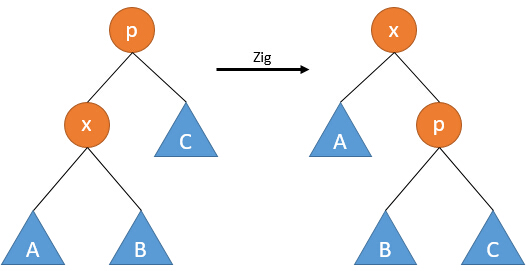
\includegraphics[width=5.5cm]{zig.jpg}
\end{center}

当$x$的父节点为根时,进行一次Zig操作。\pause
$$
\begin{aligned}
\mbox{代价}&=k+R'(x)+R'(p)-R(x)-R(p)\\
&=k+R'(p)-R(x)\\
&\le k + R'(x)-R(x)
\end{aligned}
$$
\end{frame}
\begin{frame}{splay的复杂度证明}
\begin{center}
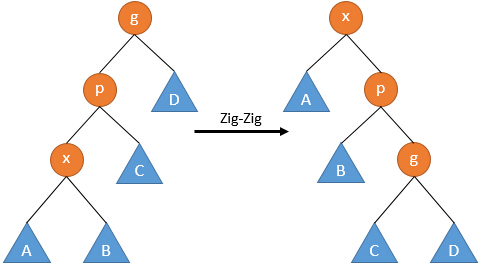
\includegraphics[width=5.5cm]{zigzig.jpg}
\end{center}

当$x$与$x$的父节点位于其父节点的同侧时,进行一次Zig-Zig操作。\pause
$$
\begin{aligned}
\mbox{代价}&=2k+R'(p)+R'(g)-R(x)-R(p)\\
&\le 2k + R'(x)+R'(g)-2R(x)\\
&=2k + 3(R'(x)-R(x)) + (R'(g)+R(x)-2R'(x))\\
&\le 2k + 3(R'(x)-R(x)) -2k\\
&=3(R'(x)-R(x))
\end{aligned}
$$
\end{frame}
\begin{frame}{splay的复杂度证明}
\begin{center}
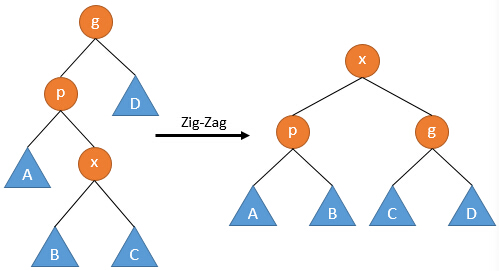
\includegraphics[width=5.5cm]{zigzag.jpg}
\end{center}

当$x$与$x$的父节点位于其父节点的异侧时,进行一次Zig-Zag操作。\pause
$$
\begin{aligned}
\mbox{代价}&=2k+R'(p)+R'(g)-R(x)-R(p)\\
&\le 2k+R'(p)+R'(g)-2R(x)\\
&=2k+2(R'(x)-R(x))+(R'(p)+R'(g)-2R'(x))\\
&\le 2k+2(R'(x)-R(x))-2k\\
&=2(R'(x)-R(x))
\end{aligned}
$$
\end{frame}
\begin{frame}{splay的复杂度证明}
综上,在一次将$x$旋转到根的操作中,均摊代价不超过$k+3(R'(x)-R(x))=O(\log n)$(注意到Zig只有不超过一次)。

把$m$次操作的均摊代价加起来,再加上不超过$n\log_2n$的初始势能,复杂度即为$O((n+m)\log n)$。
\end{frame}
\subsection{treap}
\begin{frame}{无旋treap}
对每个下标赋一个随机权值,对序列按随机权值建笛卡尔树,这就是treap的形态。\\

treap上点$i$是点$j$的祖先的概率是$\frac{1}{|i-j|+1}$,即点$i$的期望深度为$\sum_{j=1}^n\frac{1}{|i-j|+1}=O(\log n)$,因此treap的复杂度为\textbf{期望}$O(\log n)$而非\textbf{均摊},可以实现可持久化。\\

无旋treap只需要支持两种操作:分裂(split)、合并(merge)。(见板书)\\

实际上treap可以不记随机权值,在合并两棵子树$x$和$y$时,以$\frac{sz_x}{sz_x+sz_y}$的概率将$x$作为新树根。建议在可持久化treap中使用这个技巧(因为可能会复制节点,过多相同权值的节点会导致复杂度出问题)。
\end{frame}
\subsection{替罪羊树}
\begin{frame}{替罪羊树}
取一个平衡系数$\alpha \in(\frac 12,1)$,当平衡树上一个点$x$及其左右儿子$ls(x),rs(x)$满足$\max(sz_{ls(x)} + 1,sz_{rs(x)} + 1) > \alpha (sz_x + 1)$时,暴力重构整棵子树。\\

可以证明替罪羊树的复杂度是\textbf{均摊}$O(\log n)$,同时值得注意的一点是,替罪羊树的树高不超过$\log_{\frac{1}{\alpha}}n$。一般来说$\alpha$取$(0.65,0.75)$之间。

\end{frame}
\begin{frame}{替罪羊树的复杂度证明}

对节点$x$定义$\Delta(x)=|sz_{ls(x)}-sz_{rs(x)}|$,上述重构条件等价于$\Delta(x) > (2\alpha-1)(sz_x + 1)$。\\

采用势能分析。定义势能$\Phi=\frac{1}{2\alpha-1}\sum \Delta(x)$,分别讨论插入以及重构的均摊复杂度:\\

插入节点时,实际复杂度不超过当前树高,同时最多使得插入路径上所有点的$\Delta(x)$加$1$,因此均摊复杂度为$(1+\frac{1}{2\alpha-1})\log_{\frac{1}{\alpha}}n=O(\log n)$;重构子树时,

$$
\begin{aligned}
\mbox{均摊代价}&=\mbox{实际代价}+\Delta\Phi\\
&=sz_x+O(1)-\frac{1}{2\alpha-1}\Delta(x)\\
&\le sz_x+O(1)-\frac{1}{2\alpha-1}(2\alpha-1)(sz_x+1)\\
&=O(1)
\end{aligned}
$$

综上,我们即证明了替罪羊树一次插入的均摊复杂度为$O(\log n)$。

\end{frame}

\subsection{重量平衡树}
\begin{frame}{重量平衡树}
	重量平衡树一词是陈立杰在其2013年候选队论文中提出的,\sout{大家都不知道这个词具体指的是啥}。\\

	一种典型的应用是,实现一个支持$O(\log n)$插入,$O(1)$实现比较两个元素相对大小(如后缀排序)的数据结构,传统方式是$O(\log n)$地在平衡树上找到两者的位置比较,可以对平衡树的每个节点维护一个实数区间$[l,r] $,根节点的区间为$[0,1]$,每个节点的权值为$val_x=\frac{l+r}{2}$,且其左右子树的区间分别为$[l,val_x]$与$[val_x,r]$,可以发现这样比较两元素的大小就变成了比较两元素对应权值的大小,唯一的问题在于对精度的要求是关于深度的指数级别,需要使用treap或替罪羊树这种保证深度的平衡树。
\end{frame}
\subsection{CodeForces702F T-shirts}
\begin{frame}{CodeForces702F T-shirts}
\begin{block}{description}
	有$n$种T-shirts,第$i$种有价格$c_i$和品质$p_i$。
	
	有$m$个人要来买T-shirts,第$j$个人有$v_j$块钱。
	
	每个人的策略都是相同的:在自己能买得起的所有T-shirts中,买一件品质最高的,重复此过程直到买不起任何一件T-shirt。
	
	每种T-shirt每人限购一件,问最终每个人买到了多少件T-shirts。
\end{block}
\begin{block}{constraint}
	$ 1\le n, m \le 2\times 10^5, 1 \le c_i, p_i, v_j \le 10^9.$
\end{block}
\pause
\begin{block}{solution}
	对人按钱数维护平衡树,按$p_i$从大到小枚举T-shirts,问题变成每次给钱数$\ge c_i$的人答案加$1$,钱数减$c_i$。把所有人按钱数分成$3$类:$[0,c_i),[c_i,2c_i),[2c_i,+\infty)$,只需要归并前两部分后与第三部分拼接。直接暴力枚举第二部分插入第一部分,可以发现每个人只会被暴力插入$O(\log v_j)$次,因此总时间复杂度是$O(n\log n\log \max\{v_j\})$。
\end{block}
\end{frame}
\subsection{BZOJ3682 Phorni}
\begin{frame}{BZOJ3682 Phorni}
\begin{block}{description}
有一个字符串$str$和一个序列$\{a_i\}$,保证序列中的任意元素任意时刻不超过字符串长,支持以下三种操作:
\begin{itemize}
	\item 字符串前端插入新字符
	\item 单点修改序列$\{a_i\}$
	\item 询问$a_l,a_{l+1}...a_r$中的最小后缀
\end{itemize}
\end{block}
\begin{block}{constraint}
$1 \le n, m \le 5\times 10^5.$强制在线。
\end{block}
\pause
\begin{block}{solution}
所谓的后缀平衡树。

考虑插入一个新的后缀时,比它少一个字符的那个后缀已经比较过了。所以可以把当前位字符作为第一关键字,下一位后缀的大小作为第二关键字比较。再用一棵线段树维护一下询问即可。
\end{block}
\end{frame}
\section{可并堆}
\subsection{左偏树}
\begin{frame}{左偏树}
说到可并堆大家一般都写左偏树。\\

左偏树的每个节点维护了到子树内最近缺失叶子的距离$dis_x$,若该数值为$d$说明至少需要有$2^d-1$个节点,换而言之,一棵$n$个节点的左偏树中的最大$dis_x$不超过$\log(n+1)$。\\

同时,对于左偏树上的任意节点$x$满足$dis_{ls(x)}\ge dis_{rs(x)}$,因而有$dis_x=dis_{rs(x)}+1$。\\

合并两棵左偏树$A,B$时,不妨假设$A$堆顶权值大于$B$堆顶,则递归合并$B$与$A$的右子树作为$A$的新右子树。回溯时根据是否仍满足$dis_{ls(x)}\ge dis_{rs(x)}$选择性交换左右子树。\\

不难发现合并两棵左偏树时需要遍历两者的右链,由$dis_x=dis_{rs(x)}+1$可知右链长度为对数级,因此合并两棵大小分别为$n,m$的左偏树的复杂度为$O(\log(n+m))$。

(注:$\log(nm) \le \log((n+m)^2) = 2\log(n+m)$)

\end{frame}
\subsection{APIO2016 烟火表演}
\begin{frame}{APIO2016 烟火表演}
\begin{block}{description}
一棵$n$个节点的有根树,边有边权,你需要对边权进行适当修改,使得所有叶子到根的距离相等。修改的代价是原边权与现边权差的绝对值之和,你需要最小化代价和。
\end{block}
\begin{block}{constraint}
$1 \le n \le 3\times 10^5, 1 \le \mbox{边权}\le 10^9$。

\end{block}
\end{frame}
\begin{frame}{APIO2016 烟火表演}
\begin{block}{solution}
	对于一个点$u$,设$f_u(x)$表示$u$点子树内所有叶子到$u$的距离都为$x$时的最小代价,不难发现$f_u(x)$是分段一次函数,而且是下凸的。
	
	设$g_u(x)$表示$u$点子树内所有叶子到$u$的父亲距离都为$x$时的最小代价,设$u$到父亲的边权为$w$,再假设$f_u(x)$在$[L,R]$上取到最小值,考虑$g_u(x)$与$f_u(x)$的关系:
	
	$$
	\begin{aligned}
	g_u(x)=\begin{cases}
	f_u(x)+w &  x \le L\\
	f_u(L)+w-(x-L)& L < x \le L+w\\
	f_u(L)& L+w < x \le R+w\\
	f_u(L)+x-R-w& x > R+w
	\end{cases}
	\end{aligned}
	$$
	
	如果把$f_u(x)$按斜率划分成小于零、等于零、大于零的三部分,可以发现$g_u(x)$是将$f_u(x)$的第一部分全体$+w$,在一二部分之间插入斜率为$-1$的一段,并将第三部分替换成斜率为$1$的一段。用堆来维护分界点(也可以认为是函数的差分)即可。
	
	注意到$f_u(x)=\sum g_v(x)$,因此需要用可并堆实现合并。
\end{block}
\end{frame}
\section{K-D Tree}
\subsection{K-D Tree}
\begin{frame}{K-D Tree}
K-D Tree是一种基于维度划分的数据结构。\\

以2-D为例,建树时交替选择$x$或$y$坐标的中位数,将平面区域划分成两半,并左右分别递归。\\

有线段树式和平衡树式两种K-D Tree。线段树式K-D Tree只有叶子存点,在某些特定情况下实现起来更优越,缺点是常数大,且不方便插入。\\

(应该)使用更广泛的是平衡树式的K-D Tree,即每个节点都存点,需支持插入时使用替罪羊树的思想重构。\\

\end{frame}
\begin{frame}{K-D Tree}
K-D Tree被用于求解Nearest Neighbor(NN)问题的复杂度是无法保证的。
\begin{itemize}
	\item 只需要一个球就可以让它递归进每一片叶子
\end{itemize}
K-D Tree的正确用法是范围计数,比如二维的矩形修改查询、三维的立方体修改查询等。
\begin{itemize}
	\item 此时的复杂度为$O(kn^{1-\frac 1k})$,其中$k$是维数
	\item 相比于高维树套树,K-D Tree支持范围打标记,并且空间线性
\end{itemize}

当然,在随机数据下求解NN问题的效率还是很优秀的。

结论:对于不认真造数据的题目有奇效。
\end{frame}
\subsection{例题}
\begin{frame}{例题一}
\begin{block}{description}
给出一棵$n$个节点的树,每次询问或修改这样一个区域:
\begin{itemize}
	\item 在$x$点子树内,距离$x$不超过$d$的所有点
\end{itemize}
\end{block}
\begin{block}{constraint}
$1 \le n, q \le 2 \times 10^5.$
\end{block}
\pause
\begin{block}{solution}
把每个点视作二维平面上的一个点$(dfn_i, dep_i)$,那么一次操作的区域就是平面上的一个矩形。使用K-D Tree维护即可,复杂度$O(q\sqrt n)$。
\end{block}
\end{frame}
\begin{frame}{例题二}
\begin{block}{description}
有一棵树,树上的每个点都有两个权值$a_i,b_i$和一个初值为$0$的变量$x_i$,权值是不会变的,变量每天都会发生变化$x_i \gets \min(x_i+a_i, b_i)$。

每次事件会有一个发生日期,发生时会选定一个例题一中所述区域,求区域内$x_i$的和,并将区域内的$x_i$全部清零。
\end{block}
\begin{block}{constraint}
$1 \le n, q \le 2\times 10^5.$
\end{block}
\end{frame}
\begin{frame}{例题二}
\begin{block}{solution}
由于每次询问后$x_i$都会清空,答案便只与“上次修改时间”有关。

每次对一个矩形区域求答案并设置“上次修改时间”,可以在K-D Tree上定位到若干节点,从这些节点出发DFS到有标记的节点计算答案,同时回收子树内的标记。

如果一个节点上有标记,那么该节点子树内不存在标记,同时该节点子树内所有点的“上次修改时间”都相同。

这个DFS过程可以简单地分析出和普通的K-D Tree操作复杂度同级。

至于计算答案部分,每个节点的$\sum x_i$是关于修改时间的分段一次函数,可以预处理出这些分段函数,每次询问二分即可。

通过离线询问可以把二分的$\log n$去掉,复杂度为$O(q\sqrt n)$。
\end{block}
\end{frame}

\section{数据结构例题选讲}
\subsection{Luogu2839 middle}
\begin{frame}{Luogu2839 middle}
\begin{block}{description}
	定义一个大小为$k$的数集的中位数为其中第$\lfloor\frac{k}{2}\rfloor$小的数。
	
	给一个长度为$n$的序列$\{a_i\}$,$q$次询问所有左端点在$[l_1,r_1]$,右端点在$[l_2,r_2]$的区间的最大中位数。强制在线。
\end{block}
\begin{block}{constraint}
	$1 \le n, q \le 10^5, 1 \le l_1 \le r_1 < l_2 \le r_2 \le n.$
\end{block}
\pause
\begin{block}{solution}
	解决中位数一类问题的常用手段是:二分一个数$mid$,将大于等于它的设为$1$,小于它的设为$-1$,判断区间和是否$\ge 0$。
	
	那么在二分了中位数后只需要判断$[l_1,r_1]$的最大后缀和$+(r_1,l_2)$的和$+[l_2,r_2]$的最大前缀和是否$\ge 0$。
	
	二分的$mid$只可能是原序列中出现过的数,从大到小枚举,每次把一个位置从$-1$改成$1$,可以使用可持久化线段树维护。
\end{block}
\end{frame}
\subsection{HDU5709 Claris Loves Painting}
\begin{frame}{HDU5709 Claris Loves Painting}
\begin{block}{description}
给一棵$n$点的树,每个节点上有一个颜色$c_i$,$q$次询问一个点的子树中与这个点距离不超过$d$的点的颜色有多少种。

(强制在线)
\end{block}
\begin{block}{constraint}
$1 \le n, q \le 5\times 10^5.$
\end{block}
\pause
\begin{block}{solution}
按深度离线,对每种颜色维护链并(单点加,相邻LCA减),需要实现一个数据结构支持单点加以及子树(区间)求和。

(强制在线的话只需要把这个数据结构可持久化就行了)
\end{block}
\end{frame}
\subsection{CodeForces765F Souvenirs}
\begin{frame}{CodeForces765F Souvenirs}
\begin{block}{description}
给一个长度为$n$的序列$\{a_i\}$,$q$次询问区间$[l,r]$内两数差的最小值。
\end{block}
\begin{block}{constraint}
$1 \le n \le 10^5, 1 \le q \le 10^6, 0 \le a_i \le 10^9.$
\end{block}
\pause
\begin{block}{solution}
枚举$i$,考虑所有$j>i,a_j>a_i$的$(i,j)$。可能更新答案的$j$需要满足:

$$a_{j_1}-a_i>2(a_{j_2}-a_i)>4(a_{j_3}-a_i)>...$$

其中$j_x$按照下标顺序依次递增。不难发现这样的$j$只有$O(\log \max\{a_i\})$个,使用某种数据结构找出这些$j$并维护答案,可以做到$O((n\log \max\{a_i\}+q)\log n)$的复杂度。
\end{block}
\end{frame}
\subsection{CodeForces671C Ultimate Weirdness of an Array}
\begin{frame}{CodeForces671C Ultimate Weirdness of an Array}
\begin{block}{description}
给出一个长度为$n$的序列$\{a_i\}$,定义序列$\{s_i\}$的权值$val_{\{s_i\}}$为$\max_{i \neq j}\gcd(s_i,s_j)$,特别的,当$|\{s_i\}|\le 1$时,$val_{\{s_i\}}=0$。

定义$f(l,r)=\{a_1,a_2,...,a_{l-1},a_{r+1},a_{r+2},...,a_{n-1},a_n\}$,即,将$\{a_1,a_2,...a_n\}$中区间$[l,r]$移除并前后拼接后得到的序列。

求$\sum_{1 \le l \le r \le n}val_{f(l,r)}$。
\end{block}
\begin{block}{constraint}
$1 \le n \le 5 \times 10^5, 1 \le a_i \le n.$
\end{block}
\end{frame}
\begin{frame}{CodeForces671C Ultimate Weirdness of an Array}
\begin{block}{solution}
考虑计算当$val_{f(l,r)}\le i$时,每个$l$对应的右端点$r$最左能取到哪里,记为$next_l$(当不存在合法右端点时,$next_l=n+1$)。初始时$next_l=l$。

从大到小枚举$i$,考虑当限制从$val_{f(l,r)}\le i$变成$val_{f(l,r)}<i$后,哪些$next_l$会发生改变。取出所有是$i$的倍数的数的位置下标,记为$x_1,x_2,...,x_m$,因为$[l,r]$中至少要包含$m-1$个$x_i$(不然$f(l,r)$就至少是$i$了),所以$l\in(x_2,n]$内的$next_l$直接变成$n+1$,$l\in(x_1,x_2]$的$next_l$对$x_m$取$\max$,$l\in[1,x_1]$的$next_l$对$x_{m-1}$取$\max$。每次修改后统计$\sum_{l=1}^nn+1-next_l$就是满足$val_{f(l,r)}\le i$的区间数。

看上去需要$O(n\log^2n)$的吉利线段树,但实际上$next_l$是随下标单调不降的,所以取$\max$操作修改的一定是区间的一段前缀,直接做线段树区间赋值就好了,复杂度$O(n\log n)$。
\end{block}
\end{frame}
\subsection{CodeForces809D Hitchhiking in the Baltic States}
\begin{frame}{CodeForces809D Hitchhiking in the Baltic States}
\begin{block}{description}
给出$n$个区间$[l_i,r_i]$,需要确定一个序列$\{a_i\}$满足$a_i \in [l_i,r_i]$,最大化序列的LIS(最长上升子序列)。
\end{block}
\begin{block}{constraint}
$1 \le n \le 3\times 10^5, 1 \le l_i \le r_i \le 10^9.$
\end{block}
\pause
\begin{block}{solution}
考虑朴素的动态规划做法,设$f_i$表示LIS长为$i$时末尾元素的最小值。

对于新的一组$[l,r]$,找到$p=\min\{i|f_i<l\},q=\min\{i|f_i<r\}$,于是

\begin{itemize}
	\item $f_{p+1}$可以被更新为$l$;
	\item $\forall i \in[p+2,q]$,$f_i$可以被更新为$f_{i-1}+1$,由于$f_{i-1} < f_i$,等价于直接赋值。
\end{itemize}

可以发现操作实际上是把数组的一个子段平移再加$1$,此外还有$O(1)$的插入删除。使用平衡树维护即可。
\end{block}
\end{frame}


	\section{Q.\& A.}
	\begin{frame}{Q.\& A.}
	\begin{center}
		{\large 大家可以自由提问。}
	\end{center}
	\end{frame}
	\section{The end}
	\begin{frame}
		\begin{center}
			{\huge 谢谢大家!\\  \large 祝大家学业有成!}
		\end{center}
	\end{frame}
\end{document}